%PART_1_CHAP_2
\myChapter[ontexte et enjeux de la robotique à l'école]{C}{ontexte et enjeux~~\break de la robotique à l'école}
%WAIT a Review ok
\begin{resumChap}
Les notions d'open source et de robotique étant maintenant plus claires et plusieurs exemples ayant été soumis, nous aborderons dans ce deuxième chapitre les destinataires de cette technologie: les enseignants et les élèves du système éducatif français.\par%
Ainsi, nous commencerons par définir l'utilisation et l'utilisateur cible à savoir l'initiation aux sciences du numérique, les élèves et les enseignants. L'élève est en réalité une cible secondaire, c'est principalement les enseignants qui, armés de pédagogie, vont distiller ces technologies en fonction de leurs contraintes, capacités, besoins et aussi de leurs envies. \par%
Notamment, nous évoquerons les programmes officiels, la formation des enseignants, leurs contraintes de matériel ainsi que les courants théoriques de la pédagogie.\par%
Enfin, nous donnerons quelques exemples passés illustrant l'impact des nouvelles technologies dans cet écosystème.
\end{resumChap}
\section{L'utilisation cible}\label{sec:user_cible}
    \subsection{L'initiation aux sciences du numérique}
        \paragraph{L'existant}%Un enjeux sociétal
            De manière pragmatique, il est intéressant d'observer les activités qui existent déjà dans ce domaine. Ainsi la fondation \cro{la main à la pâte} propose un kit clé en main: \gui{Le projet \gui{1, 2, 3\dots codez !} vise à initier élèves et enseignants à la science informatique, de la maternelle au collège. Il propose à la fois des activités branchées (nécessitant un ordinateur, une tablette ou un robot) permettant d’introduire les bases de la programmation et des activités débranchées (informatique sans ordinateur) permettant d’aborder des concepts de base de la science informatique.}~\citeURL{123code}%%
            Nous pouvons aussi noter le projet Pixees porté par Inria et mutualisé avec le projet Class'code: \gui{Dès la rentrée 2016, Class’Code, programme de formation innovant, a pour ambition de doter les professionnels de l’éducation et de l’informatique des moyens d’initier les jeunes de 8 à 14 ans à la pensée informatique.}~\citeURL{classcode}
            Un dernier exemple, également porté par Inria, semble particulièrement intéressant car il ajoute une dimension de validation scientifique. Le projet \gui{IniRobot est une série d’activités pédagogiques destinées à la découverte de la robotique et de la programmation à l’école primaire. [\dots] IniRobot est ludique et granulaire, reposant sur des missions à réaliser avec un robot Thymio.}~\citeURL{dm1r}. Dans l'étude de Roy, D. (2015)~\citeB{roy2016inirobot} utilisant ce kit, des effets sur l’acquisition de compétences informatiques et robotiques sur des enfants de 7 à 10 ans ont été observés avec notamment une plus forte progression chez les filles. De nombreux témoignages ont relevé des effets sur l'implication des enseignants, la motivation des élèves, notamment ceux en difficulté scolaire, la diversité, et l'étendue des compétences travaillées.
        \paragraph{Quelles compétences, à quel âge.}
            Il est certain que pour s'exprimer avec aisance dans le langage informatique \tiret{et comme dans tous les langages} il faut une capacité d'abstraction élevée pour être capable de manipuler l'ensemble des concepts que ce langage permet d'exprimer. Il faut également respecter une certaine grammaire et une syntaxe afin de se faire comprendre des autres locuteurs de cette langue. Ainsi, l'approche pédagogique doit s'adapter à l'âge et au niveau de maîtrise du langage. Cependant, la difficulté et les compétences à privilégier dépendent avant tout de l'acculturation qu'a déjà l'individu sur les concepts nécessaires à la réalisation de l'activité et à l'acquisition des compétences qui y sont associées.%%
            Dés lors, un élève pourra, avec un robot, aborder facilement des notions de déplacement dans l'espace, à la maternelle, sur les concepts de référentiel égocentré et allocentré~\citeB{verjat1994confrontation}; en primaire, sur les concepts de repère et quadrillage de l'espace; au collège, sur les concepts de trigonométrie; au lycée, sur les concepts d'odométrie.%%
            D'un point de vue informatique, si un élève arrive au lycée sans jamais avoir fait de programmation, même s'il acquierera plus rapidement les notions élémentaires (car vues sous d'autres formes dans d'autres disciplines), il devra malgré tout acquérir les éléments de base du langage, comme la variable, avant de pouvoir appréhender des constructions plus complexes comme une \sht{BSM}. À l'inverse, il est tout à fait envisageable d'aborder la \sht{BSM} avec un collégien, si tant est qu'il ait manipulé et programmé fréquemment des robots en amont.%%
            C'est à l'enseignant d'adapter sa pratique aux compétences de ses élèves, quid de ses propres compétences et de ses contraintes. 
    \subsection{L'enseignant}
        Les enseignants ont des contraintes de temps et de moyens précis et très variables d’un lycée à l’autre. Afin de s’adapter au mieux à ces contraintes, il est important que les solutions proposées soient flexibles au nombre d’heures dont ils disposent, à quelle période de l’année, le niveau des élèves concernés, \etc.%%
        Les enseignants ont également des besoins et envies concernant le contenu pédagogique qui sera enseigné aux élèves. En effet, certains enseignants ont pour objectif de travailler la programmation, alors que d’autres peuvent avoir besoin d'une plate-forme robotique uniquement pour la partie découverte. De plus, au même titre que les élèves, les compétences et le niveau d’investissement et de motivation des enseignants peuvent varier. Ainsi, il faut distinguer deux postures de l'enseignant: l'apprenant face à de nouvelles connaissances et le tuteur transmettant ses connaissances.
        \citeAtion{enseigner}
        \subsubsection{Un Référentiel de compétences}
            \paragraph{Une vision institutionnelle et pragmatique}
                En 2013, le Ministère de l'Éducation Nationale renouvelle son référentiel des compétences des métiers du professorat et de l'éducation datant de 2006~\citeURL{BO-ref-prof}.Il définit 5 grands champs de compétences communes à l'ensemble du corps enseignant.
                \begin{table}[!h]
                \caption[Référentiel des compétences d'enseignement]{Référentiel de l'Éducation Nationale pour les compétences d'enseignement~\citeURL{BO-ref-prof}}
                \begin{itemize}\myItemStyle
                \item Les professeurs acteurs du service public d'éducation
                    \begin{itemize}
                    \item  Faire partager les valeurs de la République
                    \item  Inscrire son action dans le cadre des principes fondamentaux du système éducatif et dans le cadre réglementaire de l'école
                    \end{itemize}
                \item Les professeurs au service de la réussite de tous les élèves
                    \begin{itemize}
                    \item Connaître les élèves et les processus d'apprentissage
                    \item Prendre en compte la diversité des élèves
                    \item Accompagner les élèves dans leur parcours de formation \textbf{*}
                    \item Agir en éducateur responsable et selon des principes éthiques
                    \item Maîtriser la langue française à des fins de communication
                    \item Utiliser une langue vivante étrangère dans les situations exigées par son métier
                    \item Intégrer les éléments de la culture numérique nécessaires à l'exercice de son métier
                    \end{itemize}{}
                \end{itemize}
                \label{tab:BO-ref-prof}
                \end{table}
                \begin{itemize}\myItemStyle
                \item Les professeurs acteurs de la communauté éducative
                    \begin{itemize}
                    \item Coopérer au sein d'une équipe
                    \item Contribuer à l'action de la communauté éducative
                    \item Coopérer avec les parents d'élèves
                    \item Coopérer avec les partenaires de l'école
                    \item S'engager dans une démarche individuelle et collective de développement professionnel \textbf{*}
                    \end{itemize}{}
                \item Les professeurs porteurs de savoirs et d'une culture commune
                    \begin{itemize}
                    \item Maîtriser les savoirs disciplinaires et leur didactique
                    \item Maîtriser la langue française dans le cadre de son enseignement
                    \end{itemize}{}
                \item Les professeurs experts des apprentissages
                    \begin{itemize}
                    \item Construire, mettre en œuvre et animer des situations d'enseignement et d'apprentissage prenant en compte la diversité des élèves
                    \item Organiser et assurer un mode de fonctionnement du groupe favorisant l'apprentissage et la socialisation des élèves
                    \item Évaluer les progrès et les acquisitions des élèves
                    \end{itemize}{}
                \end{itemize}{}
            \paragraph{Une vision scientifique et théorique}
                Zeichner~\citeB{zeichner1983alternative} avance que l'enseignement peut se définir suivant quatre paradigmes fondamentaux qui représentent les modes de pensée actuels en matière de formation des enseignants (Calderhead ~\citeB{calderhead1992conceptualisation}):
                \begin{itemize}\myItemStyle
                    \item Le paradigme comportemental. Envisage l'enseignement comme un ensemble de capacités plus ou moins isolables à pratiquer et à maîtriser
                    \item Le paradigme artisanal. Envisage l'enseignement comme un ensemble de compétences professionnelles à acquérir sur le terrain
                    \item Le paradigme critique (orienté vers la recherche). Envisage l'enseignement comme un ensemble d'aptitudes à une investigation critique et réfléchie permettant de transformer une problématique d'enseignement
                    \item Le paradigme personnaliste. Envisage l'enseignement comme un processus de développement personnel à partir des principes et engagements particuliers propres à l'enseignant ou au futur enseignant
                \end{itemize}{}
                Paquay~\citeB{Paquay1994referentiel} représente~\citeT{tab:ref_prof} ces quatre paradigmes en établissant une correspondance avec les quatre conceptions de l'expertise professionnelle selon Kennedy ~\citeB{kennedy1987chapter} et avec les quatre dimensions de l'enseignement définies par Grootaers \& Tilman~\citeB{grootaers1991professeur}. Il dégage ainsi six ensembles de paradigmes relatifs à la nature de l'enseignement, identifiés chacun par une étiquette désignant l'enseignant:\par%
                \begin{tabular}{r p{0.65\linewidth}}
                    \gui{\textit{maître instruit}} & celui qui maîtrise des savoirs \\
                    \gui{\textit{technicien}} & qui a acquis systématiquement des savoir-faire techniques \\
                    \gui{\textit{praticien-artisan}} & qui a acquis sur le terrain des schémas d'action contextualisés \\
                    \gui{\textit{praticien réflexif}}  & qui s'est construit un \gui{savoir d'expérience} systématique et communicable \\
                    \gui{\textit{acteur social}} & engagé dans des projets collectifs et conscient des enjeux anthropo-sociaux des pratiques quotidiennes \\
                    \gui{\textit{personne}} & en relation et en développement de soi
                \end{tabular}\par%
                \begin{table}
                \centering
                \caption[le métier d'enseignant et la formation, Paquay~\citeB{Paquay1994referentiel}]{Conceptions, objectifs et stratégies pour le métier d'enseignant et la formation, Paquay~\citeB{Paquay1994referentiel}}
                \label{tab:ref_prof}
                \begin{minipage}{0.95\linewidth}
                    \centering
                    \subcaption{Conceptions diverses du métier d'enseignant et de la formation des enseignants}
                    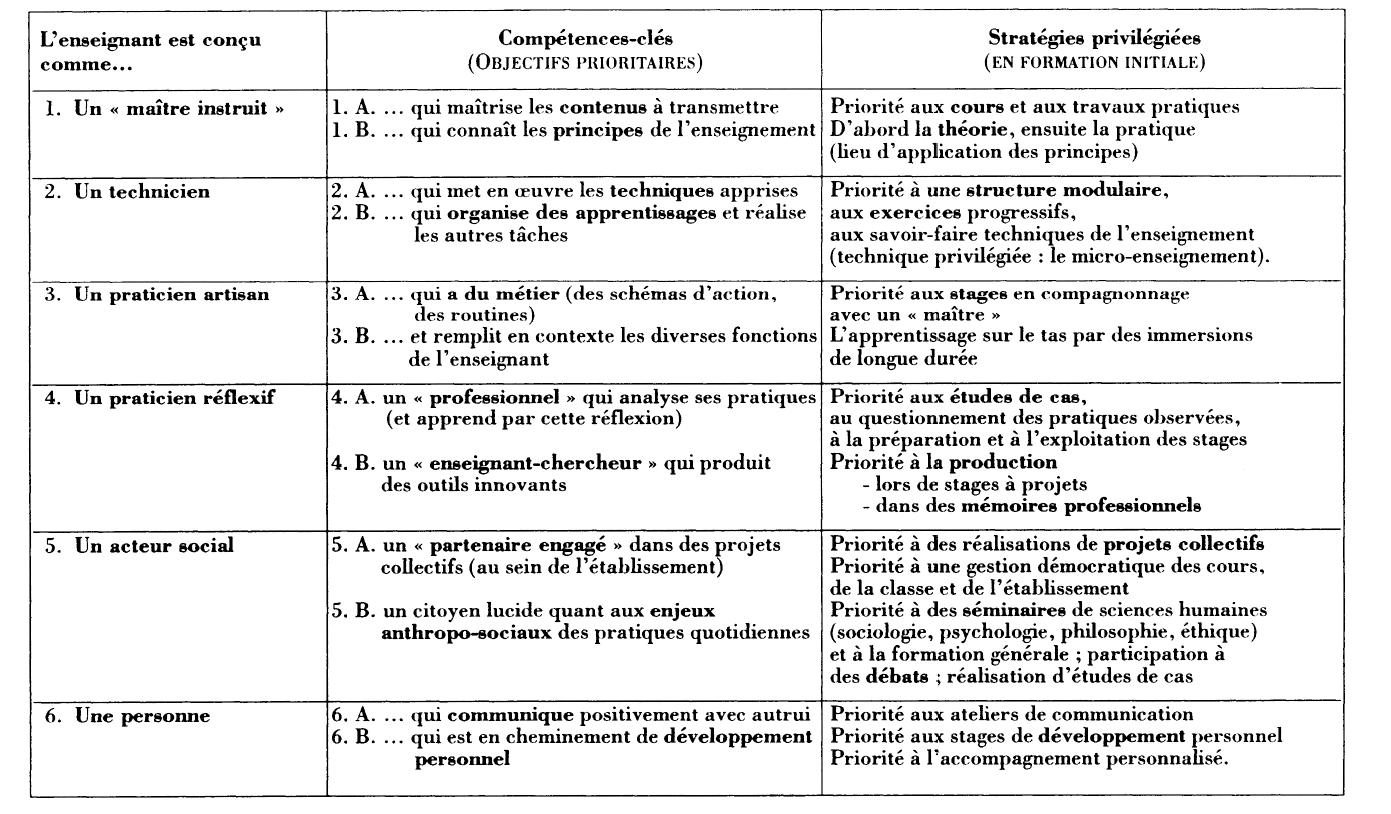
\includegraphics[width=\linewidth]{Figures/paquay-ref_con_prof.png}
                    \label{tab:ref_con_prof}
                \end{minipage}
                \begin{minipage}{0.95\linewidth}
                    \centering
                    \subcaption{Objectifs et stratégies privilégiés pour chaque conception du métier d'enseignant}
                    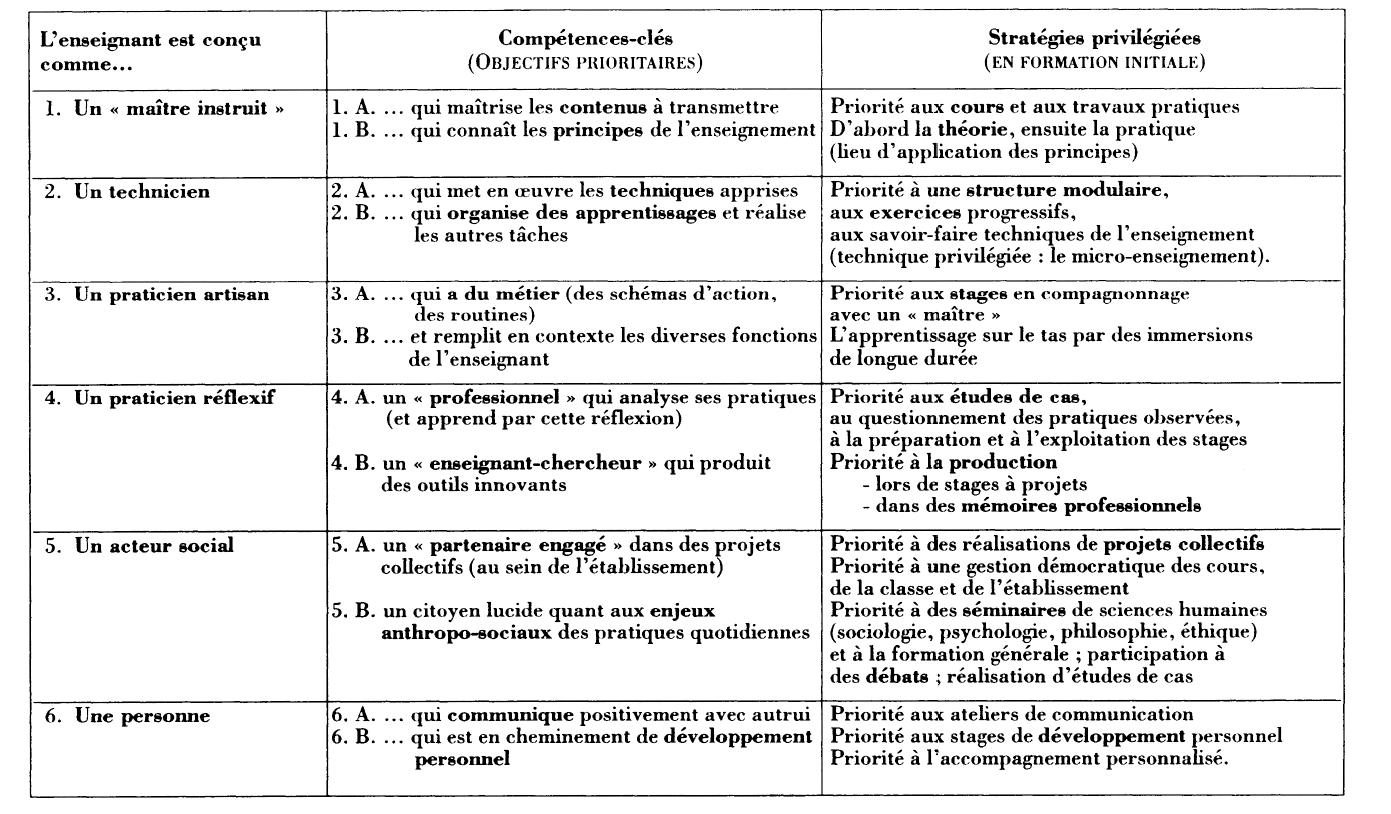
\includegraphics[width=\linewidth]{Figures/paquay-ref_con_prof.png}
                    \label{tab:ref_obj_prof}
                \end{minipage}
                \end{table}
        \subsubsection{Sur le terrain}
            \paragraph{En tant que tuteur}
                Un enseignant est un instituteur (du latin \textit{institutor} \gui{celui qui dispose, administre}), un précepteur (du latin \textit{praeceptor} \gui{celui qui enseigne, maître}) d'un enseignement (du latin \textit{insignis}, remarquable, marqué d'un signe, distingué) qui est chargé de transmettre des connaissances ou méthodes de raisonnement à autrui. Pour ce faire, il se conduit simultanément comme un tuteur (du latin \textit{tutor}, dérivé de \textit{tueor} \gui{regarder fixement, avoir à l’œil}, d’où \gui{surveiller, protéger} ), un pédagogue (du latin \textit{paedagogus} \gui{qui marche avec}), ou un éducateur (du latin \textit{educo} \gui{élever, nourrir, produire}). Il dispose d'une grande liberté d'action dans le choix et la constitution de ses ressources, tout en devant respecter un programme et des objectifs officiels~\citeS{sec:programme-officiel}. Pour cela, il a lui-même été formé~\citeS{sec:formation} et continue de l'être afin d'actualiser son socle de connaissances (théoriques et pratiques).
            \paragraph{En tant qu'apprenant}
                C'est souvent dans les coulisses de la classe que l'enseignant trouve l'occasion d'accroître ses compétences, que ce soit par la formation continue ou auto-formation~\citeS{sec:auto-formation}. En classe, devant les élèves, il reste \cro{le détenteur} du savoir, \cro{la référence}. Même si de nombreux enseignants tentent de faire tomber cette barrière en favorisant l'implication et l'autonomie de ses élèves, la gestion de la classe impose à l'enseignant de \cro{garder le contrôle} le mettant dans une situation où il a tendance à rester dans sa zone de confiance. Ainsi, dans le cadre des nouvelles technologies, nous constatons que la majorité des enseignants n'ont pas eu accès dans leur formation initiale à des enseignements sur le numérique; que le temps et les formations continues disponibles pour ce sujet ne sont pas suffisants; et que dans le même temps, la population d'élèves manipule ces outils depuis leur plus jeune âge. De fait, l'expertise des élèves est plus grande, cependant celle-ci se fonde sur l'expérience et les usages et non sur la réflexion et l'analyse. Ainsi, l'enseignant doit à la fois acquérir les compétences nécessaires à forger son expertise de façon rigoureuse et savoir comprendre puis, le cas échéant, démonter les fausses croyances que l'élève a pu développer par sa pratique du numérique.
    \subsection{Les élèves}
        Tous les étudiants valident en fin de 3\ieme un socle commun de connaissances, de compétences et de culture qui comprend le B2i, remplacé progressivement par PIX en 2018~\citeS{sec:certif}.%, des  pour la culture informatique et quelques exercices en \sht{scra} pour la programmation. 
        D'autres sections, au lycée, permettent d'approfondir ces domaines comme avec l'option \sht{ICN}.
        Cependant, les niveaux restent très hétérogènes, selon l’environnement des élèves, leurs centres d’intérêt, leur implication dans l’utilisation des réseaux sociaux, \etc. Leur motivation à participer à ce projet peut également énormément varier d’un individu à l’autre. De plus, les lycéens peuvent être parfois très habiles pour utiliser des outils numériques, faisant souvent preuve d’une très grande dextérité, sans pour autant connaître le fonctionnement ni les enjeux sous-jacents. De plus, le caractère multi-disciplinaire de la robotique force à utiliser plusieurs types de compétences difficilement synthétisables dans un seul individu. Dès lors, le travail en groupe devient indispensable (et permet de réduire les coûts matériels).
        \paragraph{En équipe projet}
            Avoir un objectif concrêt, favoriser l'autonomie des élèves dans la définition de celui-ci et dans les moyens à mettre en œuvre pour le réaliser, tout en constituant une équipe hétérogène mais complémentaire d'individus, semble être la pratique la plus efficace pour favoriser la motivation et la réussite des élèves sur un spectre large de compétences. Cependant, ce type de projet est d'une part, difficile à mettre en place de manière systématique du fait des contraintes horaires et, d'autre part, cela demande à l'enseignant beaucoup de flexibilité mentale pour suivre et accompagner l'ensemble des projets de ses équipes.
        \paragraph{En groupe de TD}
            Actuellement une grande majorité des activités en robotique se réalise en groupe. D'un point de vue pédagogique cette organisation durant un \sht{TD} semble être la plus adaptée, comparativement, au travail individuel~\citeS{sec:peda_edu}. Cependant, il est à craindre, qu'à l'instar des recherches qui s'effectuaient dans les années 90, en groupe, au \sht{CDI}, avec un unique ordinateur à se partager, les activités robotiques ne se transforment en travail individuel avec l'accroissement des ressources matérielles à disposition.
            Concernant la programmation, de nombreux enseignants, non avertis et sous la pression des programmes, se contentent de mettre en place des solutions telles que \sht{scra} pour initier à la logique informatique lorsque de nombreuses ressources d'activités débranchées permettent d'aborder ces mêmes notions, mais, de façon concrète et en groupe.
    \subsection{L'utilisateur cible}
        Faciliter les apprentissages des utilisateurs consultant nos ressources est un objectif fondamental. Bien qu'il vise l'initiation aux sciences du numérique, et \textit{in fine} les élèves, l'utilisateur cible est adulte. En effet, dans l'environnement scolaire, il est rare d'atteindre directement et massivement les élèves. Les contenus et ressources disponibles sont d'abord évalués par l'enseignant, puis, s'il les juge pertinents les pratique et se les approprie, enfin il les réutilise \etou les modifie pour les intégrer à ses propres contenus. C'est uniquement à cette étape que l'élève rentre en contact avec la ressource. Ainsi, l'objectif est d'avantage de fournir aux enseignants des exemples d'utilisation plus que de prescrire des usages \etou ressources \cro{clé en main} pour l'élève. L'enseignant est donc l'unique vecteur institutionnel pour toucher les élèves. Plus généralement, ce constat peut être étendu à l'ensemble des activités éducatives (qui par définition requièrent un tuteur, un animateur, \etc) car, de fait, les élèves vont s'orienter préférentiellement vers du contenu étiqueté \cro{récréatif} que vers du contenu étiqueté \cro{éducatif}. 
\section{L'environnement scolaire}
    \subsection{Le programme officiel}\label{sec:programme-officiel}
        \myPhantom{paragraph}{Introduction}
            L'éducation nationale propose via les programmes scolaires un certain nombre de directives et d'axes d'enseignement. Ceci nous permet de cadrer les différents objectifs éducatifs que doivent chercher à atteindre les séquences pédagogiques proposées aux lycéens. En effet un certain nombre de notions et de compétences doivent être acquises par l'apprenant et seront évaluées à plusieurs niveaux: d'abord par le contrôle continu proposé par l'établissement et ensuite de manière officielle et nationale via différents examens ( \eg BAC). 
            Ainsi l'un des premiers travaux réalisé par l'équipe a été d'analyser ces directives. En est ressorti un document permettant de cadrer à la fois le public visé et les objectifs à atteindre. Notamment les programmes scolaires officiels ont été recompilés sous forme de diagramme offrant une meilleure lisibilité.
        \paragraph{De nombreuses réformes}
            Depuis 1802 et Loi générale sur l'instruction publique, de nombreuses réformes ont jalonné l'histoire de l'Éducation Nationale~\citeURL{Frise-educ}. Quasi annuelle, seules quelques réformes ont bouleversé le fonctionnement de l'École de la République: 
            1975: la réforme Haby;
            1982: Alain Savary, \gui{la rénovation du collège unique};
            1989: la loi \gui{Jospin}, la loi d'orientation sur l'éducation;
            1993-2005: de François Bayrou à Ségolène Royal;
            2005: François Fillon, la loi d'orientation pour l'avenir de l'école;
            2009: Luc Chatel et la réforme du lycée;
            2013: Vincent Peillon, la loi de refondation de l'École de la République;
            2013: la réforme des rythmes scolaires;
            2016: Najat Vallaud-Belkacem et la réforme du collège;
            2018: Jean-Michel Blanquer et \gui{l'École de la confiance}
            (source \textit{rue des écoles}\citeURL{reforme}).%%
            Concernant notre projet deux réformes ont joué un rôle prépondérant: \href{http://www.Éducation.gouv.fr/pid285/bulletin_officiel.html?cid_bo=100720}{le Plan \cro{numérique à l'école}}~\citeURL{planNum} en 2012 participant à sa réussite, et la réforme de 2019 sur le BAC 2021 qui compliqua considérablement la mise en place des expérimentations longitudinales. Notons également, qu'en 2019, la réforme sur \gui{l'École de la confiance} propose dans son chapitre 2 (article 38~\citeURL{loi-confiance}) de facilité l'accès à l'école aux scientifiques, constituant un terrain d'expérimentations écologiques~\citeS{sec:adm}.
        \paragraph{En 2012}
            Avec l’entrée des Sciences du Numérique dans les programmes de l'enseignement scolaire en France, la question des approches et des outils pertinents pour ces nouveaux enseignements se pose. 
            Ce contexte est favorable pour explorer la création et l’intégration d’un nouvel outil robotique destiné à épauler ces nouvelles connaissances à acquérir.
            Depuis la rentrée 2012-2013, l'enseignement de spécialités \sbg{ISN} est proposé aux élèves de terminale de la série scientifique (élèves de 17 à 18 ans)~\citeB{dowek2012informatique} au même titre que les enseignements déjà mis en place, de spécialité de mathématiques, sciences physiques et chimiques ou sciences de la vie et de la terre (\cf \href{http://eduscol.Éducation.fr/cid59678/presentation.html}{Eduscol, Pr{\'e}sentation \sht{ICN}}~\citeURL{ICN-prez}).
            Par ailleurs, \href{http://www.Éducation.gouv.fr/pid285/bulletin_officiel.html?cid_bo=100720}{le Plan \cro{numérique à l'école}}~\citeURL{planNum}, lancé par le président Hollande en mai 2015 pour faire entrer les élèves de plain-pied dans le monde numérique et pour favoriser les usages pédagogiques du numérique, devait équiper les collèges de ressources matérielles et pédagogiques, et créer de nouveaux enseignements de l'école primaire (élèves de 6 à 10 ans) au secondaire (élèves de 11 à 15 ans). Dans ce cadre, l'enseignement d'exploration \sht{ICN} (Informatique et Création Numérique) a été mis en place dans quelques lycées en classe de seconde (15 ans) en septembre 2015 puis généralisé à la rentrée 2016 (\cf \href{http://www.Éducation.gouv.fr/pid285/bulletin_officiel.html?cid_bo=100720}{Bulletin Officiel}~\citeURL{ICN-BO}) et étendu en 1ère (16 à 17 ans) et terminale (17 à 18 ans) aux sections L (littéraire) et ES (économique et social) en 2016. En effet, deux heures hebdomadaires de cet enseignement sont proposées dans les classes de première (16 à 17 ans) des séries générales (S, ES et L) pour permettre aux élèves qui le souhaitent d'acquérir une meilleure maîtrise des concepts mis en œuvre dans le domaine du numérique.
            \begin{table}
                \centering\label{tab:prog_ICN}
                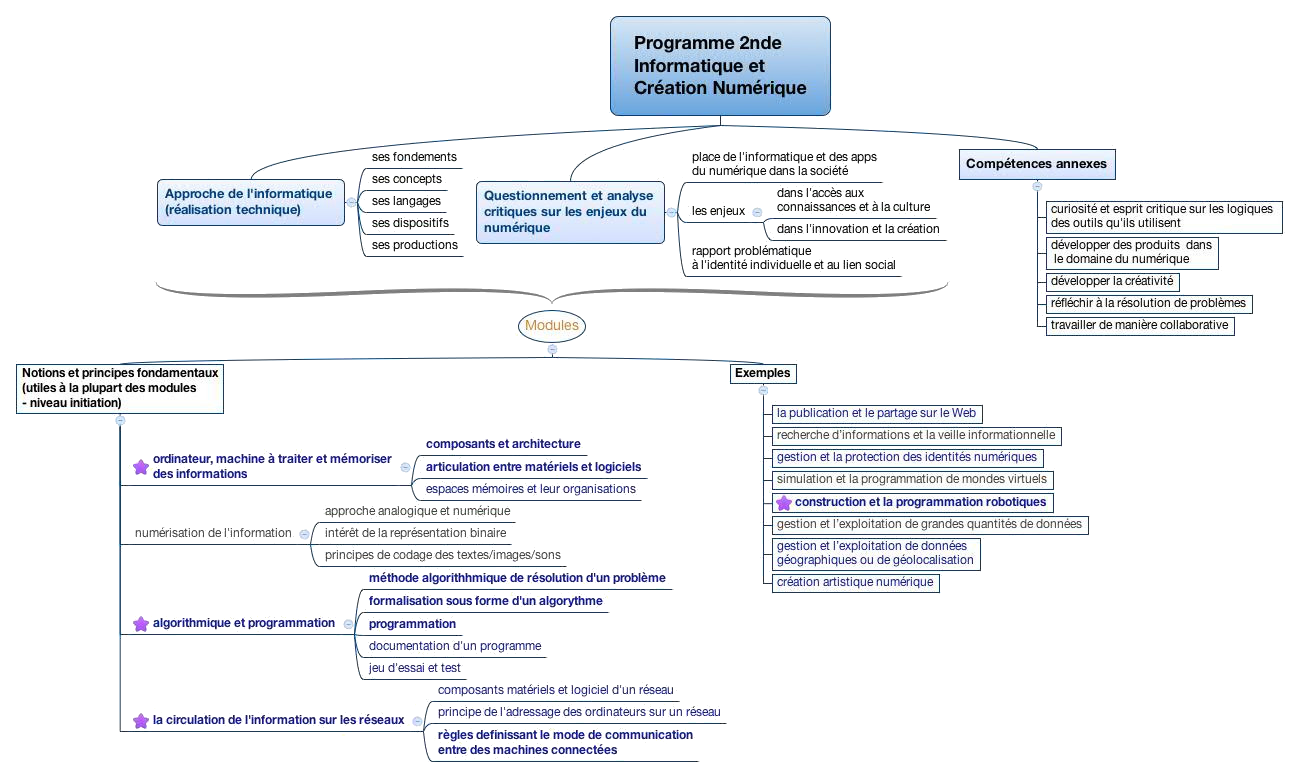
\includegraphics[width=0.9\linewidth]{Figures/Programme_2nde_ICN_.png}
                \caption[Programme \textit{ICN}, Noirpoudre~\RI]{Schéma du programme de l’enseignement de spécialité de seconde \sht{ICN},~\citeR{Noirpoudre}.}
            \end{table}        
            \begin{table}
                \centering\label{tab:prog_ISN}
                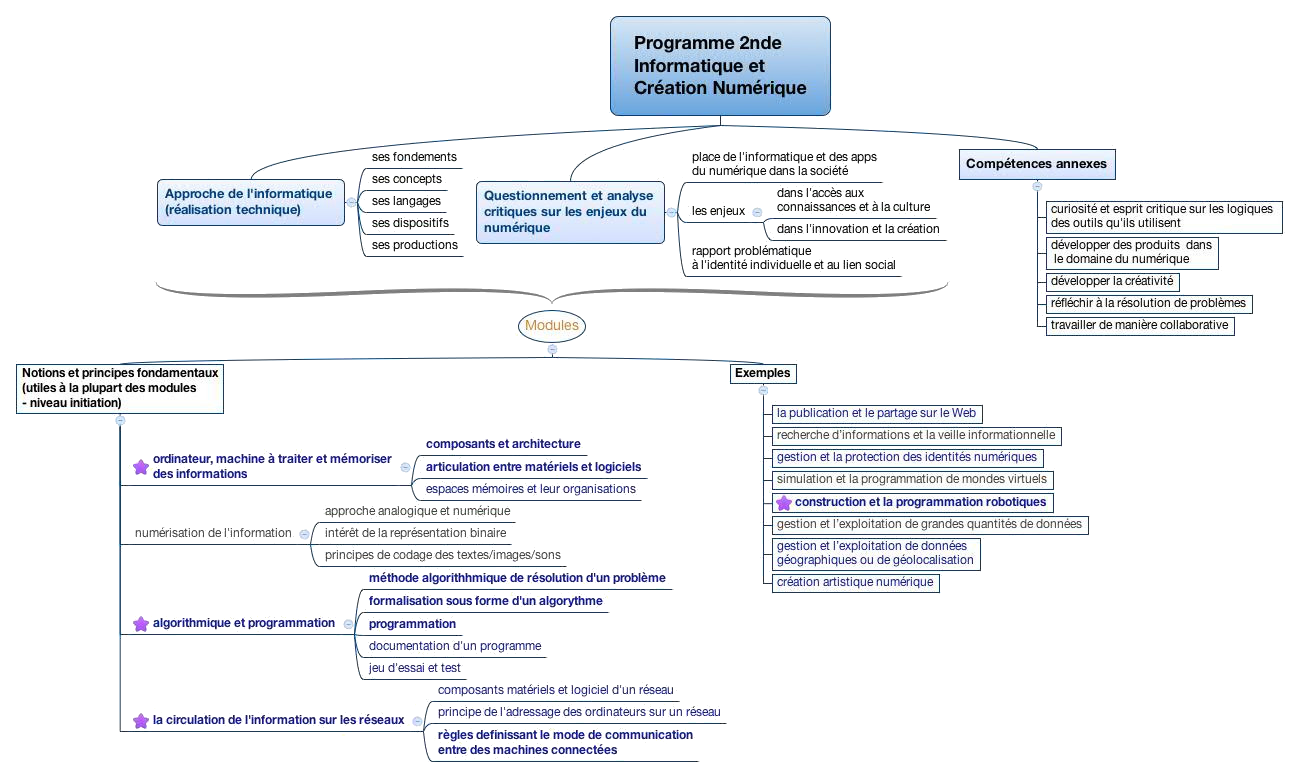
\includegraphics[width=0.9\linewidth]{Figures/Programme_2nde_ICN_.png}
                \caption[Programme \textit{ISN}, Noirpoudre~\RI]{Schéma du programme de l’enseignement de spécialité de terminale \sht{ISN},~\citeR{Noirpoudre}.}
            \end{table}\par%
            \myPhantom{subparagraph}{ISN}
                En ce qui concerne \sht{ISN}, cet enseignement est proposé en classe de terminale de spécialité scientifique à raison de 2 heures par semaine. Il offre une introduction à la science informatique (information numérique, algorithmique, langages de programmation, architectures informatiques, représentation de l'information numérique, \etc) pour comprendre les usages (internet, réseaux sociaux, \etc), les créations (objets numériques, représentations 3D, \etc) et les applications logicielles. 
                Pour y parvenir, une pédagogie de projet et un travail pluridisciplinaire sont privilégiés avec une progression pédagogique pouvant alterner différents types d'activités (l'acquisition de nouveaux savoirs, exposés, projets, \etc). Par ailleurs, un projet de groupe, souvent réalisé au second semestre, est à présenter au baccalauréat pour être ensuite évalué, avec un coefficient 2, au cours d'une épreuve orale.~\citeURL{ISN-prog}
            \myPhantom{subparagraph}{ICN}
                Quant à l’option facultative \sbg{ICN}, cet enseignement d'exploration est proposé en classe de seconde générale et technologique à raison d'1h30 par semaine et constitue également une initiation au numérique. En plus de vouloir amener les élèves à comprendre que leurs pratiques numériques quotidiennes sont rendues possibles par une science informatique rigoureuse, il apporte des éléments de réflexion autour des enjeux sociétaux qui en découlent. À l'instar de l'enseignement \sht{ICN} et comme son intitulé \cro{Création Numérique} l'indique, une mise en activité est privilégiée à un enseignement purement théorique.
                Par ailleurs, le programme officiel laisse la liberté aux enseignants de proposer les modules de leur choix. Un module est décrit comme une progression d'activités, permettant la découverte des notions, principes et outils nécessaires à l'élaboration du projet. Toutefois, certaines notions et principes sont fondamentaux, utiles à la plupart des modules, et s'articulent autour de quatre thèmes: l'ordinateur, machine à traiter et mémoriser des informations; la numérisation de l'information; l'algorithmique et la programmation; la circulation de l'information sur les réseaux. (\cf \href{https://www.legifrance.gouv.fr/eli/arrete/2017/7/4/MENE1719956A/jo/texte/fr}{programme officiel}~\citeURL{ICN-prog})
                Comme c'est une option facultative et de découverte, il n'y a pas de cadre d'évaluation imposé en \sht{ICN}, contrairement à l'enseignement de spécialité \sht{ISN}.
        \paragraph{En 2019}\label{sec:ref_2019}
            \gui{Il n'y aura plus de série en voie générale mais des parcours choisis par chaque lycéen en fonction de ses goûts et de ses ambitions.
            Le baccalauréat 2021 reposera pour une part sur un contrôle continu (40\prc) et pour une autre part sur des épreuves terminales (60\prc)} voilà ce qu'on pouvait lire sur education.gouv.fr le 11/06/2019~\citeURL{Bac2021-web}.
            En terminale, deux épreuves écrites portant sur les enseignements de spécialité auront lieu au printemps, plus un oral (d'une durée de 20 minutes). Les deux épreuves de philosophie se dérouleront en juin. Et, les épreuves anticipées de français se dérouleront comme aujourd'hui en fin de première.
            Le contrôle continu sera composé d'épreuves communes organisées pendant le cycle terminal.
            L'organisation du lycée général et technologique, comme les programmes d'enseignements, évolueront pour préparer au nouveau baccalauréat.
            Le lycée offrira trois types d'enseignements:
            \begin{itemize}
                \item Un socle de culture commune (français, mathématique, histoire, \etc)
                \item Des disciplines de spécialités choisies par l'élève (3 disciplines en 1\iere puis 2 en terminale). Ces disciplines, comme \sht{NSI}, bénéficient d'un quota horaire supérieur.
                \item Des enseignements facultatifs permettront à l'élève de compléter son parcours.
            \end{itemize}
            Des enseignements nouveaux permettant aux élèves de \gui{partager une culture scientifique, d'apprendre à coder et de comprendre les grands défis du monde contemporain} ont été annoncés.
            Pour garantir l'égalité entre les candidats et les établissements scolaires, une \cro{banque nationale numérique de sujets} sera mise en place, les copies anonymes seront corrigées par d'autres professeurs que ceux de l'élève.%%
            Dès Février 2019 une plaquette officielle~\citeURL{Bac2021-pdf} concrétisait la mise en place de ce nouveau BAC et donc les interrogations quant à la mise en place des nouveaux programmes publiés en janvier 2019 pour les secondes~\citeURL{Bac2021-BO-seconde} (applicable en septembre) et en juillet 2019 pour les terminales~\citeURL{Bac2021-BO-ter} (applicable en 2020).%%
            Nous pouvons souligner la disparition des sections \sht{ISN} et \sht{ICN} au profit d'un enseignement de tronc commun \gui{sciences numériques et technologie}~\citeURL{Bac2021-prog-scd} portant sur 6 thématiques: Internet; Le Web; Les réseaux sociaux; Les données structurées et leur traitement; Localisation, cartographie et mobilité; Informatique embarqué et objets connectés; La photographie numérique. Et d'un enseignement de spécialité \gui{numérique et sciences informatiques}~\citeURL{Bac2021-prog-ter} préconisant une démarche de projet: il est organisé autour de huit rubriques, mais il ne constitue cependant pas un plan de cours; il appartient aux professeurs de choisir leur progression parmi ces 8 thèmes: Histoire de l’informatique; Représentation des données (types et valeurs de base); Représentation des données (types construits); Traitement de données en tables; Interactions entre l’homme et la machine sur le Web; Architectures matérielles et systèmes d’exploitation; Langages et programmation; Algorithmique.
        \paragraph{Impact sur le projet}
            Bien qu'il semble facile d'établir des parallèles entre les nouveaux et les anciens programmes, il y a une réelle nécessité de reconstruction des matériaux pédagogiques. 
            D'une part, car ce mécanisme de sélection de 3 options en 1\iere puis 2 en terminale fait craindre aux enseignants (des filières numériques) que les \cro{bons élèves} fassent un choix du type \cro{maths - physique - numérique} en 1\iere puis, en terminale, abandonnent \cro{numérique} sous la pression des filière post-bac, dégradant ainsi le niveau de la filière numérique. De plus, aujourd'hui, un élève s'engageant en \sht{ICN} continue en \sht{ISN}, ainsi de nombreux enseignants ont construit leurs ressources sur une perspective d'un enseignement de 2ans. Or, avec ce nouveau système, les enseignements de seconde et de 1\iere doivent potentiellement se suffire à eux-mêmes. 
            D'autre part, il y a nécessité de reconstruction, car l'enseignement des sciences du numérique était auparavant réservé à des filières spécialisées, demain, il se démocratise et se retrouve au programme de l'ensemble des élèves de seconde. Ceci nécessite des ressources humaines supplémentaires pour enseigner ces nouvelles notions. 
            De plus, la charge de travail supplémentaire de création / redéfinition des contenus scolaires, qui est allouée à l'enseignant n'est pas répercutée dans son quota horaire.
            Dans ce contexte, il est aisé de comprendre que les enseignants partenaires du projet Poppy~Éducation n'avaient à disposition le temps suffisant pour intégrer les contraintes d'un protocole scientifique dans leurs enseignements en pleine mutation: la majorité mettant à l'épreuve leur propre contenu durant cette période~\citeS{sec:limit_proto}.
        \paragraph{La certification}\label{sec:certif}
            Actuellement les compétences numériques - outre les filières post-bac ou de spécialisation - sont actées par le \textit{B2i} puis le \textit{C2i} (Brevet/Certification Informatique et Internet). En 2017, le ministère créa par arrêté un nouveau groupement d’intérêt public: Gip~Pix. Gip~Pix doit assurer le portage de la nouvelle plateforme en ligne d’évaluation et de certification des compétences numériques \textit{PIX}~\citeURL{pix} qui se substituera progressivement au \textit{B2i} dès la rentrée 2017-2018.
            Les épreuves évalueront les connaissances mais également les savoir-faire et \gui{la capacité à identifier les enjeux du numérique}. Des modalités innovantes d’évaluation seront proposées, privilégiant des activités réalisées dans leur environnement numérique réel: interactions, manipulations de  fichiers, résolutions de problèmes, productions créatives, évaluations par les pairs, \etc.
            Quatre grandes thématiques sont proposées: Informations et données; Communication et collaboration; Création de contenu; Protection et sécurité. Elles sont divisées en 7 à 9 étapes qui permettent une certification progressive des compétences.
    \subsection{Le matériel}\label{sec:materiel}
        \myPhantom{paragraph}{Introduction}
            L'enseignement des sciences du numérique, comme toute discipline, a ses propres caractéristiques nécessitant des outils et des méthodes pédagogiques adaptées répondant aux spécificités de ces nouveaux programmes. 
            Par ailleurs, ces enseignements s'exerçant dans un environnement bien spécifique influant sur la manière d'enseigner et les choix d'outils à utiliser, il est important de prendre en considération les particularités et les contraintes de la salle de classe traditionnelle. 
            Ces nouvelles exigences demandent aussi aux enseignants de s'adapter rapidement en se formant, en créant de nouvelles séquences d'activités et en s'équipant en matériel.
        \paragraph{Budgets}
            Les nombreux échanges avec les enseignants partenaires ainsi que les réponses à un questionnaire donné au début et à la fin des expérimentations a permis de mettre en évidence certains besoins et contraintes~\citeS{sec:ucd}.
            Dans cette analyse, nous avons notamment remarqué des contraintes budgétaires: dans le système éducatif français, l'état ouvre généralement des options avec peu de ressources financières attribuées. Néanmoins, en anticipant suffisamment, il est possible de monter un projet et de demander des subventions à la région par exemple ou de demander à son établissement, sur fonds propres, bien que le budget de celui-ci soit généralement assez restreint.
            À noter, qu'il semble plus facile d'obtenir un budget auprès de son établissement ou de la région si l'enseignant est familiarisé avec la technologie et peut montrer des résultats concrets. Par exemple, un enseignant travaillant depuis un an avec les robots Poppy ErgoJr a vu sa demande d'achat d'un robot Poppy Torso (un torse humanoïde venant de la plateforme Poppy ErgoJr, permettant de faire des projets pédagogiques complexes mais d'un prix beaucoup plus élevé) facilement acceptée.
        \paragraph{Mise à disposition}
            Dans ce contexte et durant la phase de développement, il semblait donc indispensable de pouvoir proposer une mise à disposition du matériel prototypé: avoir en prêt des robots peut permettre d'étaler les achats sur plusieurs années afin de diminuer les coûts et donc de pouvoir faire une commande plus rapidement. En effet, pour travailler avec le robot Poppy ErgoJr en classe (sans utiliser le robot virtuel), il est souvent nécessaire de faire une commande de plusieurs robots (souvent 3 ou 4 par an), ce qui est vrai pour de nombreux autres robots. Par exemple: deux enseignants d'un même établissement, auquel le projet Poppy Éducation avait prêté 8 robots Poppy ErgoJr, ont pu se faire financer par leur établissement 4 robots ErgoJr pour la première année d'utilisation des robots en classe. Ce qui leur a permis d'avoir deux flottes de 6 robots à faire circuler dans les classes, et de pouvoir renouveler des achats les années suivantes.
            Durant la phase d'évaluation et de dissimulation ce procédé de mise à disposition du matériel sous forme de prêt gracieux fut conservé. Cependant, ce système implique la mise en place d'un contrat de collaboration entre les établissements scolaires partenaires et Inria~\citeA{pdf:contrat}. De plus, tous les projets ne peuvent pas se permettre ce genre de système, mais il se révèle comme un atout facilitateur.
        \paragraph{Intégration}
            Concernant les contraintes liées à la salle de classe, des enseignants rencontrent des difficultés sur le terrain liées au réseau informatique de l'établissement.
            \subparagraph{Le réseau informatique des établissements}\label{sec:connect_classe}
                Ils n'ont pas tous accès au compte administrateur des ordinateurs (gestion rectorale) et sont souvent limités dans l'installation des outils. De plus, la manière dont le réseau informatique de l'établissement fonctionne varie d'un établissement à l'autre.
                Les ordinateurs des écoles fonctionnent sous un système d'exploitation Windows, et parfois GNU/Linux. Ils sont connectés au réseau via un câble Ethernet, et ne disposent généralement ni de Wifi ni de Bluetooth par mesure de prévention contre l'exposition des enfants aux ondes électromagnétiques. 
                De plus, l'installation de tout logiciel sur les ordinateurs est soumise à une demande administrative complexe où une personne du service informatique de l'académie doit se rendre dans l'établissement pour faire la manipulation.
                Détail supplémentaire, le réseau de l'établissement passe par un proxy national qui est utilisé pour filtrer les sites accessibles ou non aux élèves.
                En utilisant ce proxy, le temps de résolution DNS peut impacter fortement le trafic. Ainsi, en utilisant la résolution d'un nom de domaine d'une machine du réseau local avec le protocole mDNS peut prendre plus de 5 secondes.
                Si la machine ne réponds pas, le time-out est extrêmement long (nous avons mesuré plus de 30s dans un établissement) ce qui provoque une page qui charge dans le vide et met beaucoup de temps avant d'afficher une erreur. Des solutions à ces problèmes ont donc dû être trouvées~\citeS{sec:devellopement}.
                Par ailleurs, le programme laissant libre, à l'enseignant, d'utiliser les outils de son choix, nous avons déterminé plusieurs facteurs entrant en jeu dans les choix des enseignants, comme leurs compétences et leurs préférences (par exemple, un enseignant choisit le langage de programmation Java car c'est le langage qu'il connaît le mieux ou parce qu'il le trouve plus pertinent), mais aussi les compétences des élèves et les outils auxquels ils sont déjà familiarisés  ainsi que les technologies accessibles dans leur établissement.
                Il y a aussi une tendance des enseignants à vouloir utiliser des objets où les éléments sont visibles et accessibles pour pouvoir travailler dessus.
    \subsection{La formation}\nocite{kim2015robotics}
        %De ce fait, nous avons également identifié des besoins en formation. 
        \paragraph{La formation continue}
            Le plan de formation des enseignants de l'option \sht{ICN} et \sht{ISN}  est à la libre initiative de chaque académie sous la responsabilité du recteur. Concernant la région de la Nouvelle-Aquitaine, une formation académique optionnelle de trois jours est proposée une fois par an, incluant \sht{ICN} et \sht{ISN}, pour introduire les contenus, faire passer des idées générales à transmettre aux élèves et faire découvrir des outils aux enseignants. Cette formation relève principalement d'une initiation et les enseignants partenaires ont exprimé la nécessité de formations plus spécifiques, de besoins en ressources pour se former et d'activités à proposer à leurs élèves, telles quelles ou à modifier. Sur ce dernier point, nous avons remarqué l'envie des enseignants de s'approprier les ressources pour les adapter selon les besoins et leurs compétences initiales.
        \paragraph{La formation initiale}\label{sec:formation}
            Dès la rentrée scolaire 2019, le nouveau référentiel de formation intitulé \cro{Former l'enseignant du \siecle{21}} des futurs professeurs des premiers et seconds degrés et CPE sera mis en œuvre.
            \begin{figure}[!h]
            \begin{minipage}{0.55\linewidth}
                \centering
                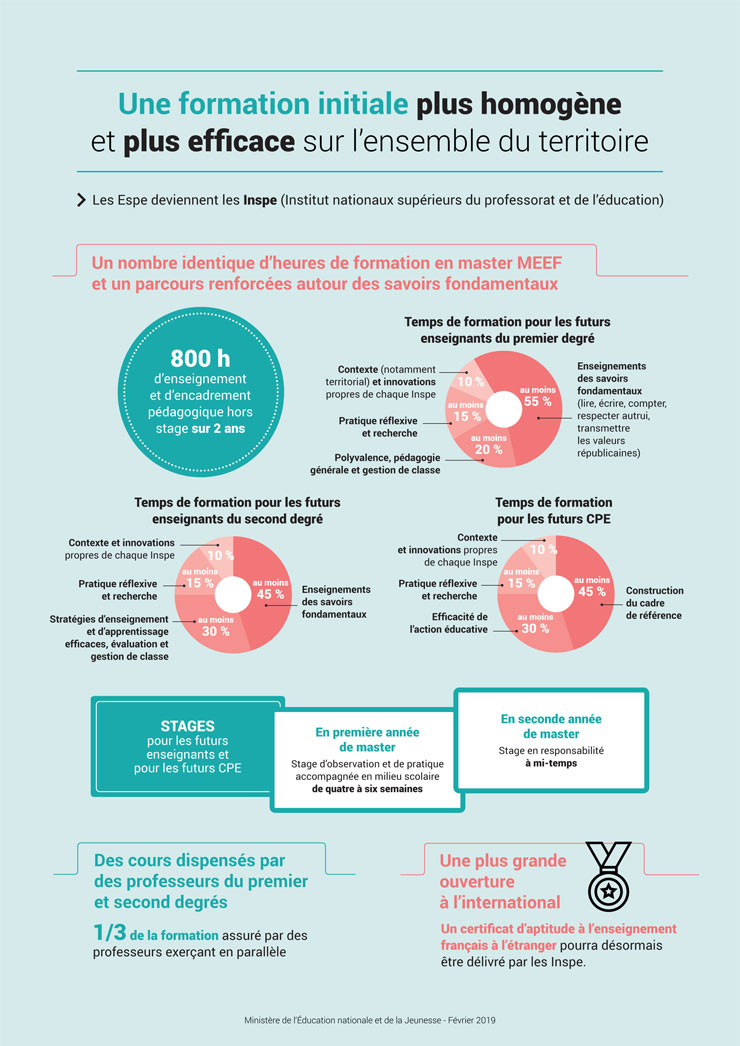
\includegraphics[width=\linewidth]{Figures/gouv_Formation_Inspe_1150278.jpg}
                \caption{Présentation formation initiale des enseignants en 2019}
                \label{fig:formation_prof}
            \end{minipage}
            \hfill
            \begin{minipage}{0.43\linewidth}
            \myDefautStyle
                Il définit le contenu de la formation délivrée au sein des \sbg{INSPE}. Si le futur enseignant ou personnel d'éducation doit être conscient du niveau élevé de responsabilités qu'il aura à assumer quotidiennement, il doit d'abord être formé à l'exercer pleinement. Ce référentiel de formation précise les objectifs, axes de formation, les compétences travaillées, et leurs niveaux de maîtrise attendus en fin de master MEEF.
                Dans le référentiel adjoint à cette réforme plusieurs mentions (principalement la CC9) sont faites sur les usages du numérique~\citeS{sec:ref_2019}.
            \end{minipage}
            \end{figure}\par%
             Cependant, il faudra attendre plusieurs années avant que les élèves d'aujourd'hui (formés aux outils du numérique) ne deviennent eux-mêmes enseignants et plusieurs décennies pour qu'ils soient majoritaires dans le corps enseignant. D'où l'importance du besoin d'actualisation des connaissances, par les voies officielles et la formation continue, ou, via des moyens personnels et l'auto-formation.
        \paragraph{L'auto-formation}\label{sec:auto-formation}
            \subparagraph{Par nécessité}
                L'auto-formation est valorisée dans ce nouveau référentiel (en P14) par cette mention: \gui{Culture de l’apprentissage tout au long de la vie, notamment grâce aux outils numériques et à la mobilité}
                Mais cela relève déjà d'une nécessité pour les enseignants qui souhaitent respecter les programmes ou simplement pour ceux souhaitant que leurs enseignements s'intègrent dans des usages modernes.  
            \subparagraph{Le volontariat}
                L'accessibilité du savoir est croissant, hier l'imprimerie, puis Encarta, Wikipédia, aujourd'hui les \sht{MOOC}~\citeS{sec:mooc}. Ainsi, de nombreux individus se retrouvent face à un grand nombre de possibilités de développement professionnel et personnel. Sur cette base de volontariat intrinsèquement motivante~\citeF{fig:motiv1}, l'individu capitalise ces nouvelles compétences en les intégrant dans sa pratique globale.
    \subsection{La pédagogie}\label{sec:peda_edu}
        \subsubsection{Le vecteur de la pédagogie}
            \paragraph{Pas intrinsèquement lié avec l'outil}
                L'outil en lui-même ne possède pas intrinsèquement une visée pédagogique. Celle-ci est relative à l'usage qui sera fait de l'outil. En revanche, cet outil possède un certain nombre de caractéristiques qui lui sont propres et qui favorisent certains types d'usages. Par exemple, un outil tel qu'un stylo permet de stocker une quantité d'information limitée à la taille de son support (le papier) mais qui permettra sont
                stockage à long terme. D'un autre coté, une craie ne permettra pas de stocker durablement une information mais permettra sa réécriture à l'infini. En revanche, il n'y a pas de différence entre une ardoise blanche - feutre noir et une ardoise noire - craie blanche. La pédagogie viendra de comment sont exploitées ces caractéristiques pour atteindre l'acquisition d'une compétence: pour un exercice d'entraînement aux opérations mathématiques, nul besoin de stocker à long terme, en revanche les théorèmes permettant leur résolution, oui.
                Ainsi, l'outil doit posséder suffisamment d'affordance pour faciliter son appropriation par l'identification et la maîtrise de ses caractéristiques.
            \paragraph{Véhiculé par l'enseignant}
                C'est au cours de sa formation, puis par son expérience que l'enseignant apprend à maîtriser l'ensemble des outils à sa disposition pour réaliser sa mission. C'est lui, directement en contact avec les élèves, qui retranscrit les prescriptions sociétales faites sur ses objectifs. Il garde en tête les principes didactiques de sa discipline, les notions et compétences qu'il a à transmettre, mais il n'appartient qu'à lui de sélectionner telle ou telle pratique pédagogique tant que leur validité continue de faire débat.
        \subsubsection{Plusieurs courants de pensée}
            La pratique pédagogique est une chose extrêmement personnelle, pourtant elle se base sur des conceptions communes mais implicites car totalement intégrées par le pédagogue. Selon Marguerite Altet~\citeB{altet2013pedagogies}, on retrouve habituellement les mêmes cinq éléments: l'apprenant, l'enseignant, le savoir, la communication, la situation; avec une finalité différente pour l'élève et l'enseignant qui sont: \Li apprendre, se socialiser, s'épanouir, s'autonomiser, et \ii instruire, éduquer, former. De là, on classe les diverses pédagogies en trois ou quatre types.
            \paragraph{Les pédagogies traditionnelles}
                Représentent la vision centrée sur l'enseignant détenteur du savoir universelle. L'objectif est la transmission du contenu déjà structuré par assimilation passive de l'élève. C'est la vision dominante jusqu'au \siecle{19} elle est notamment défendue par les congrégations religieuses (les jésuites, \etc).
            \paragraph{Les pédagogies actives} 
                Cette vision est centrée sur l'élèves acteur de la construction de son savoir. c'est lui qui s'approprie par développement personnelle les connaissances et les procédures.
                Ce mouvement émerge avec des auteurs comme John Dewey (1897)~\citeB{chen1958doctrine} et la pédagogie Fonctionelle; Adolphe Ferrière (1899)~\citeB{adolphe1922ecole}, Ovide Decroly (1921) et  l'école nouvelle; Célestin Freinet (1924)~\citeB{freinet1969pour} et 
                la pédagogie coopérative, ou encore la pédagogie de la liberté pour Roger Cousinet (1959)~\citeB{cousinet1950education}.
            \paragraph{Les pédagogies technologiques}
                Ce type de pédagogie se centre essentiellement sur les moyens techniques et opératoires (techno-centrisme) pour permettre à l'élève d'acquérir efficacement des savoirs, savoir-faire, savoir-être, en temps voulu. Il se développe particulièrement suite à la mise en évidence du conditionnement dit opérant par Thorndike~\citeB{thorndike1898animal} à la fin du \siecle{19} puis généralisé par Skinner~\citeB{skinner1963operant} au court du \siecle{20}. L'élève est acteur de son apprentissage au sens où il reconstruit un savoir programmé par suite de renforcements. %On parle également de pédagogie par objectifs  qui articule objectif- méthode- évaluation- objectif dans une optique de rationalisation et d'efficacité
            \paragraph{Les pédagogies socialisées}
                On parle ici de socio-centrisme, c'est à dire que l'enfant est vu comme un membre de la communauté sociale. L'objectif est d'éduquer socialement cet élève, de former un homme social, un citoyen. On y retrouve des conceptions comme celle de A. Makarenko (marxiste) en 1917~\citeB{vexliard1951education}, la pédagogie institutionnelle de Fernand Oury~\citeB{oury1967vers}, la pédagogie progressiste de G. Snyders~\citeB{snyders1976ecole}
            \paragraph{Autres courants}
                Certaines pédagogies sont difficilement classables, car à cheval sur plusieurs conceptions. Par exemple, Lev Vygotski~\citeB{vygotskiui1997pensee} propose en 1934 une vision socio-constructiviste qui repose sur l'idée selon laquelle l'acquisition durable des connaissances par l'enfant (pédagogie active) est favorisée par la prise en compte du champ social dans lequel il est situé (pédagogies socialisées). Ou, 
                Maria Montessori~\citeB{montessori2013montessori} en 1907 et sa pédagogie éponyme.
                Elle repose sur l'éducation sensorielle et kinesthésique de l'enfant (pédagogie active)  via un set d'outils spécialement conçus (pédagogies technologiques). 
                D'autres existent encore, telles les pédagogies cognitives. Ces pédagogies sont basées sur les recherches en psychologie cognitive, qu'elles utilisent afin de rendre l'enseignement plus efficace \etou efficient. Elles utilisent notamment les recherches sur la mémoire, la méta-cognition et l'expertise pour déduire des méthodes et pratiques pédagogiques adaptées. Parmi ces pédagogies, on trouve notamment la pédagogie explicite, et l'apprentissage multi-épisodique d'Alain Lieury~\citeB{lieury2013motivation}.
        \subsubsection{Faits \& mythes en éducation}
            Même si chaque pédagogue à une pratique particulière qui jongle entre les différents cadres théoriques proposés par de nombreux auteurs, certains faits ou mythes sont aujourd'hui démontrés. Ainsi, peu importe le cadre, ces notions restent vraies et doivent toujours orienter la pratique. Dans son ouvrage \gui{Les neurosciences en éducation} Gros, Hippolyte~\citeB{gros2018neurosciences} nous dénombre quelques uns de ces faits:
            \paragraph{Les mémoires}
                Il n'existe pas \cro{une} bonne ou \cro{une} mauvaise mémoire, en revanche on peut distinguer plusieurs types de mémoires: la mémoire dite sensorielle, elle stocke toutes les informations sensorielles mais de manière extrêmement transitoire; la mémoire de travail, elle traite des informations de différentes natures pendant quelques dizaines de secondes mais seules sept informations peuvent être maintenues et manipulées en même temps~\citeB{miller1956magical}, elle est très sensible aux interférences de l’environnement. La mémoire déclarative, d'abord sémantique qui contient l’ensemble des faits et des connaissances acquises au cours de la vie. Sa capacité ne semble pas limitée et les informations peuvent y être maintenues pendant toute une vie, même si elles sont sujettes à l’oubli. Ensuite, la mémoire déclarative épisodique, elle, contient l’ensemble des événements (multimodale) liés à notre histoire personnelle et sa capacité: nos souvenirs. Elle est moins sujette à l’oubli notamment quand les souvenirs sont chargés d’émotion. Enfin, la mémoire procédurale qui, contrairement au deux précédentes, est implicite, stock toutes les procédures, routines et automatismes développés au fur et à mesure de nos apprentissages (\eg marcher, écrire, faire du vélo, \etc) cette mémoire demande un long entraînement et beaucoup de répétitions mais ne souffre pas (ou très peu) de l'oubli.\par%
                Cependant, cela ne tient que pour cette mémoire, en règle générale, la répétition massée (rabâcher une information de nombreuses fois en un temps court pour la mémoriser) n’est efficace qu’à très court terme (ou dans la nécessité d'un apprentissage \cro{par cœur}). À noter, que le fait d'apprendre par cœur ne \cro{muscle} pas le cerveau, la mémoire n’est pas un muscle unique et le fonctionnement des mémoires est complexe. Cependant on remarque qu'il existe une spécialisation dans la nature du signal traité (mots, formes, visages, couleurs, odeurs, \etc) qui pourra conduire à un filtrage plus ou moins conscient chez l'individu.
                Pour une bonne mémorisation de la connaissance, on passe d'abord par une phase de découverte / manipulation, puis une phase de généralisation des observations qui permettra de générer une représentation mentale de la notion devenue concept. Ensuite, pour une bonne assimilation (à long terme) s'en suivra plusieurs périodes d'atténuation puis de reconstruction amenant progressivement vers une consolidation de la connaissance.\par%
                Une fois une connaissance acquise, la supprimer par le simple fait de la volonté paraît inconcevable en l’état actuel des recherches. Cependant, on oublie, les recherches s'axent plutôt sur l’inhibition et la réorganisation du cerveau avec des processus nécessitant de l’entraînement et donc du temps.
                %Par ailleurs, comme vu dans le premier point, la rémanence d’un souvenir dépendra beaucoup de l’émotion (agréable ou désagréable) associée: oublier un souvenir dont la charge émotionnelle est forte paraît impossible.
                %Encore une fois, tout dépend du type d’information: une information dans la mémoire de travail est vite oubliée (surtout s’il y a des distractions dans l’environnement au moment de l’encodage) mais une information stockée dans la mémoire procédurale semble presque ineffaçable.
                On oublie, et parfois on brode: un souvenir est une reconstruction et cette reconstruction est souvent biaisée, involontairement \etou volontairement, par des ajouts \etou des modifications. Nous sommes tous tentés de combler des trous par des éléments qui nous paraissent plausibles (mais qui ne sont pas forcément véridiques). Ainsi, il faut perpétuellement remettre en cause ses connaissances et le cas échéant les réactualiser.
            \paragraph{Le cerveau}
                Une conception courante est l'existence de gens au \cro{cerveau gauche} ou au \cro{cerveau droit}.
                Les compétences qui permettraient d’attribuer à un individu des qualités (logique pour les cerveaux gauches et créativité pour les cerveaux droits) ne sont pas clairement associées à un hémisphère plutôt qu’un autre sur le plan biologique.
                Chacun apprend de manière plus efficace selon son mode préféré (visuel, auditif, kinesthésique). Pour autant, il n'existe pas de profil visuel/ auditif/ kinesthésique.
                Aucune étude n’a été capable de montrer que le mode préféré de l’apprenant conduit à une efficacité plus grande en termes d’apprentissage ou de mémorisation. Il peut exister des préférences des élèves mais préférence n’est pas synonyme d’efficacité supérieure.\par%
                Un autre mythe régulièrement cité concerne la sous utilisation de notre cerveau (environ 10\prc), or tous les neurones du cerveau humain servent à quelque chose\dots mais effectivement, ils ne sont pas tous activés en même temps, mais, de la même façon qu'un feu tricolore n'utilise pas seulement 1/3 de ses capacités sous prétexte qu'une seule lumière s'active à la fois, on ne peut pas réduire l'activité globale à l'activation d'un système à un instant T.
                On ne peut pas non plus réduire le développement socio-cognitf d'un individu à une période: non, tout ne se joue pas avant 6 ans (ni avant 2, 3, 4, ni après, 10 ou 25 ans). En revanche, on remarque qu’il existe des périodes de plus ou moins grande plasticité cérébrale, durant lesquelles le cerveau peut se reconfigurer plus rapidement à la suite d’apprentissages. La neuroplasticité est possible à tous les âges de la vie, le développement cognitif est très dynamique et se caractérise par des phases de progression, de stagnation et de régression.\par%
                Enfin, il est également souvent rapporté que le bilinguisme freine le développement des capacités langagières de l’enfant, or aucune étude ne tranche actuellement la question. Le développement des compétences langagières des enfants dépend d’un nombre important de variables: âge, taux d’exposition, nature de l’apprentissage (immersion, apprentissage volontaire, par écran ou en interactions physiques), nature des langues parlées, \etc. En revanche, l’acquisition précoce et simultanée de deux langues semble développer certaines capacités cognitives comme les fonctions exécutives qui rendraient donc, sur le long terme, de tels apprentissages plus pertinents. Plus généralement, l’apprentissage entremêlé (deux thèmes différents, deux types d’exercices différents, deux matières différentes, \etc) est plus efficace pour la mémorisation à long terme car l’attention requise est importante pour passer de l’un à l’autre. L’effort déployé en mode apprentissage entremêlé à des effets positifs à long terme, mais ralentit l'acquisition à court terme.
            \paragraph{Les préjugés}
                Une déclaration bien connu de tous: \gui{les garçons sont meilleurs en maths que les filles} pourtant, les études à la fois sociologiques et scientifiques ont montré qu’il n’y a aucun lien entre le sexe et les performances en mathématiques.
                Si les filles se sentent moins attirées par les maths que les garçons, la cause n’en est pas neurobiologique mais culturelle: les stéréotypes influencent les goûts plus qu’on ne veut le croire.\par%
                Plus généralement, certaines pseudosciences tendent à vouloir valider l'un ou l'autre des mythes ici énoncés: non, la Brain Gym (ou kinésiologie) ne muscle pas le cerveau; non, les fleurs de Bach ne favorisent pas le sommeil ou les apprentissages; non, la loi de l’attraction (pensée positive) ne fera pas de vous un génie, même en y croyant très fort. Ce sont des pseudosciences: elles sont appelées ainsi car elles se revendiquent être  des sciences, pourtant elles ne respectent pas le processus scientifique qui consiste à mettre à l’épreuve des données expérimentales méthodologiquement recueillies, sur la base d’un test statistique inférentiel. La science se différencie de la pseudoscience dans le sens où les scientifiques sont toujours prêts à remettre en cause leurs résultats et la véracité des connaissances en doute quand une nouvelle observation contradictoire surgit.
\section{Les nouvelles technologies}\label{sec:honeyBee}
    Historiquement, on voit au sein des établissements scolaires l'entrée progressive des technologies dites nouvelles. Une technologie est nouvelle à un instant T, puis elle se banalise. Ainsi, un simple téléphone ou un photocopieur ont, en leur temps, été de nouvelles technologies ayant impacté significativement les pratiques de l'école.
    \subsection{Impact sur l'école}
        \paragraph{Les salles informatiques des années 90}
            Récemment, une avancée majeure concerna l'accès direct à l'information. Dans les années 80 et 90 le développement rapide des micro-ordinateurs et la réduction des coûts ont permis son implantation dans les établissements scolaires. Des programmes dédiés, tant côté matériel (langage de programmation, bureautique, encyclopédie, logiciels pédagogiques divers, \etc) que du côté institutionnel (avec la spécification de certaines notions et compétences à acquérir) ont vu le jour. Cependant, très vite plusieurs interrogations se sont posées quant à l'intérêt pédagogique que ces innovations devaient créer, notamment concernant une intégration de l'informatique via la mise en place de salles informatiques spécialisées qui, in-fine, pourrait menacer les innovations qu'elles sont censées annoncer~\citeB{watson1990classroom}.
        \paragraph{Connexion Internet des années 2000}
            Nous observons le même constat dans les années 2000 avec la généralisation de internet (haut debit) d'abord un engouement certain puis une suite d'interrogations~\citeB{maddux1994internet}. Il est souvent fait la critique que les enseignants, non avertis à ces nouvelles technologies, y soient réfractaires. Cependant, il semblerait qu'il s'agisse plus d'une volonté de rester sur des bases qui leurs sont connues et solides. Mais, avec un accompagnement adapté, ils semblent tout à fait prompts à utiliser ces technologies~\citeB{schofield1997internet}.
        \paragraph{Les tablette et TBI des années 2010}
            Plus récemment, avec l'arrivée des \sht{TBI} on observe là encore les mêmes schémas. De nombreuses publications, plutôt positives ont pullulé au cours des années 2010, aujourd'hui les discours sont plus nuancés~\citeB{smith2005interactive}: le \sht{TBI} n'ayant pas montré de différence significative dans l'évolution des apprentissages. Cependant, l'aspect attirant, engageant, motivant qu'engendre ce dispositif est vécu comme un effet positif par les enseignants et les élèves, même si ils ne sont que subjectifs ou in-quantifiables.
            %Cette volonté de rester sur des choses connues peut s'avérer une bonne stratégie, notamment quand le mésusage d'une technologie devient délétère aux innovations qu'elle annonce. Typiquement le gain de temps que doit dégager un TBI de par son utilisation et souvent compensé par les problèmes techniques, ou pire 
    \subsection{L'effet \textit{lune de miel}}
        C'est un phénomène bien connu de l'arrivée d'une nouvelle technologie dans un secteur: elle suscite l'engouement.
        On parle d'effet \cro{lune de miel}~\citeB{csad2012honeymoon}. Celui-ci crée chez l'utilisateur un désir de la découverte issu de sa curiosité naturelle. Cependant, ce sentiment est éphémère, et il arrive fréquemment que cette technologie nouvelle devienne vite désuète, banalisée. Dés lors, la motivation qui était galvanisée, va peu à peu s'estomper.
        Cet attrait de la technologie et de la nouveauté peut biaiser les résultats observés, ainsi McDougall~\citeB{mcdougall2001guest} donne, en 2001, des indications sur les méthodes d’évaluation préconisées: il précise que les démarches d’évaluation des dispositifs incluant des technologies doivent se distancer des modèles classiques comparant des groupes expérimentaux avec des groupes contrôles par le biais d'expérimentations à long terme et en contexte. Cependant, il est parfois pertinent de mener des passations \cro{traditionnelles} permettant de préciser ou de mettre en évidence certains effets, même pour des nouvelles technologies.